\documentclass[main.tex]{subfiles}
\begin{document}



\section{Metrieken op $\mathbb{R}^p$}
\label{sec:metr-op-mathbbrp}

\subsection{De gewone metriek op $\mathbb{R}^p$}
\label{sec:gewone-metriek-op}

\begin{vb}
  $\mathbb{R}^{p}$, uitgerust met de volgende functie als metriek, is een metrische ruimte:
  \[ d:\ \mathbb{R}^{p}\times\mathbb{R}^{p}\rightarrow (x,y) \mapsto d(x,y)=\|x-y\| \]
  We noemen dit de \term{gewone metriek} of \term{euclidische metriek} op $\mathbb{R}^{p}$.
  \extra{bewijs}
  \begin{figure}[H]
    \centering
    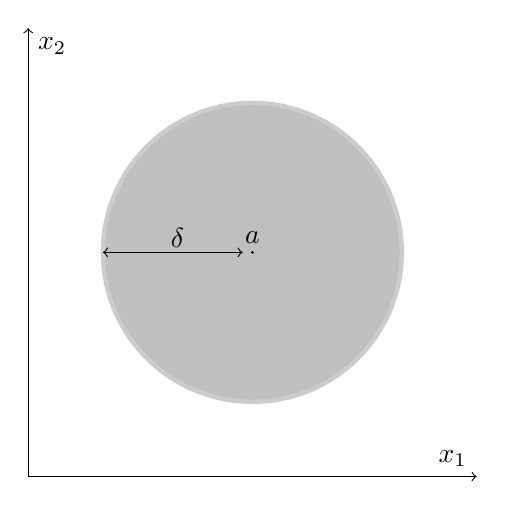
\begin{tikzpicture}
      \begin{axis}[ 
        ticks=none,
        axis lines = middle,
        axis line style={->},
        ymin=0, ymax=3,
        xmin=0, xmax=3,
        xlabel={$x_{1}$},
        ylabel={$x_{2}$},
        axis equal image,
        disabledatascaling
        ]
        \filldraw [ultra thick,fill=black!25!white, draw=black!20!white] (1.5,1.5) circle [radius=1];
        \fill [fill=black] (1.5,1.5) circle [radius=0.01];
        \draw (1.5,1.6) node {$a$};
        \draw (1.5,1.5) node {} edge[<->] (0.5,1.5);
        \draw (1,1.6) node {$\delta$};
      \end{axis}
    \end{tikzpicture}
    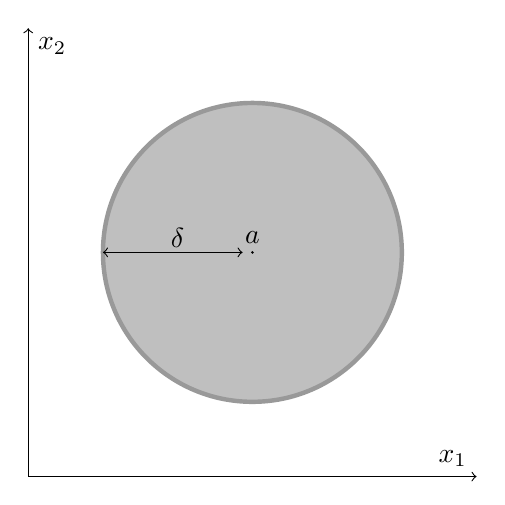
\begin{tikzpicture}
      \begin{axis}[ 
        ticks=none,
        axis lines = middle,
        axis line style={->},
        ymin=0, ymax=3,
        xmin=0, xmax=3,
        xlabel={$x_{1}$},
        ylabel={$x_{2}$},
        axis equal image,
        disabledatascaling
        ]
        \filldraw [ultra thick,fill=black!25!white, draw=black!40!white] (1.5,1.5) circle [radius=1];
        \fill [fill=black] (1.5,1.5) circle [radius=0.01];
        \draw (1.5,1.6) node {$a$};
        \draw (1.5,1.5) node {} edge[<->] (0.5,1.5);
        \draw (1,1.6) node {$\delta$};
      \end{axis}
    \end{tikzpicture}
    \caption{Een open bol en een gesloten bol in $\mathbb{R}^{2},d$}
  \end{figure}
\end{vb}

\begin{vb}
  $\mathbb{R}^{p},d$ is separabel door $\mathbb{Q}^{p}$.
\extra{bewijs}
\end{vb}

\begin{st}
  \examenvraag{TTT II 2014}
  Zij $A$ en $B$ twee niet-lege, onderling disjuncte delen van $\mathbb{R}^{p}$ met $p \ge 2$ en benoem $\delta$ als volgt:
  \[ \delta = \inf \{ \|a-b\| \mid a\in A, b\in B \} \]
  \begin{enumerate}
  \item Als $A$ en $B$ beide gesloten en begrensd zijn, geldt $\delta > 0$.
  \item Geef expliciete tegenvoorbeelden als \'e\'en van de voorwaarden niet geldt.
  \item Argumenteer of dit resultaat valt te verheffen naar willekeurige metrische ruimten.
  \end{enumerate}

  \begin{klad}
    Allereerst moeten we een idee krijgen van wat $\delta$ precies voorstelt.
    Het ziet ernaar uit dat $\delta$ voorstelt wat we de ``afstand'' tussen twee vlakke figuren zouden noemen.
    Intu\"itief kennen we natuurlijk enkel de afstand voor wat we ``normale'' figuren zouden noemen.
  \end{klad}

  \begin{enumerate}
  \item
    \begin{klad}
      Intu\"itief: De verzameling $V = \{ \|a-b\| \mid a \in A, b \in B \}$ zal gesloten en (naar onder) begrensd zijn als zowel $A$ als $B$ begrensd is.
      Van een gesloten en begrensde verzameling weten we dat het infimum erin zit.
      Omdat de verzamelingen $A$ en $B$ disjunct zijn, kan $0$ geen element zijn in die verzameling $V$.
    \end{klad}
    \begin{proof}
      Bewijs uit het ongerijmde: stel dat $\delta$ niet strikt positief is.\\
      Strikt negatief kan $\delta$ niet zijn, want normen zijn positief.
      Stel daarom dat $\delta$ nul is.
      Omdat $V$ een begrensde verzameling is, bestaat het infimum.
      Het infimum is dan een element van $\overline{V}$\waarom
      \TODO{het infimum van een begrensde verzameling behoort tot de sluiting ervan}
      Omdat $\delta$ tot $\overline{V}$ behoort, bestaat er een rij $(z_{n})_{n}$ in $V$ die naar $\delta$ convergeert.\prref{pr:metrische-ruimte-sluiting-itv-limiet}
      De rij $(z_{n})_{n}$ kunnen we beschrijven als $(\|a_{n}-b_{n}\|)_{n}$ met $(a_{n})_{n}$ en $(b_{n})_{n}$ respectievelijk rijen in $A$ en $B$.
      Omdat $A$ en $B$ gesloten en begrensd zijn, bestaan er een convergente deelrijen $(a_{n_{k}})_{k}$ en $(b_{n_{k}})_{k}$ van respectievelijk $(a_{n})_{n}$ en $(b_{n})_{n}$.\stref{st:in-rp-gesloten-en-begrensd-itv-rijen}
      Noem $a$ en $b$ de respectievelijke limieten van deze deelrijen.
      De limiet van $(\|a_{n_{k}}-b_{n_{k}}\|)_{k}$ is dan $|a-b|$.\waarom
      Dit is bovendien ook de limiet van $(\|a_{n}-b_{n}\|)_{n}$.\stref{st:in-rp-deelrij-zelfde-limiet}
      Omdat $|a-b|$ nul is, moeten $a$ en $b$ gelijk zijn.\deref{de:norm}
      Dit is in tegenspraak met de disjunctheid van $A$ en $B$.
      Contradictie.
    \end{proof}
  \item
    \begin{itemize}
    \item Als $A$ en $B$ niet begrensd zijn (maar wel gesloten) kan $\delta$ nul zijn.
      \begin{proof}
        Kies $A$ en $B$ als volgt:

        \noindent
        \begin{minipage}{.45\textwidth}
          \begin{figure}[H]
            \centering
            \begin{tikzpicture}
              \begin{axis}[ 
                ticks=none,
                axis lines = middle,
                axis line style={->},
                ymin=-3, ymax=3,
                xmin=0, xmax=10,
                xlabel={$x_{1}$},
                ylabel={$x_{2}$},
                axis equal image,
                disabledatascaling
                ]
                \addplot[name path=A1,color=red,thick,domain=0.1:9]{1/x};
                \addplot[name path=A2,color=white,domain=0.1:9]{3};
                \addplot[red!20] fill between[of=A1 and A2];
                \addplot[name path=B1,color=blue,thick,domain=0.1:9]{-1/x};
                \addplot[name path=B2,color=white,domain=0.1:9]{-3};
                \addplot[blue!20] fill between[of=B1 and B2];
                
                \draw (1.5,1.5) node {$A$};
                \draw (1.5,-1.5) node {$B$};
              \end{axis}
            \end{tikzpicture}
          \end{figure}
        \end{minipage}
        \begin{minipage}{.45\textwidth}
          \[ A = \left\{ \left(r,+q\right) \ \middle|\  r \in \mathbb{R}_{0}^{+}, q\in \mathbb{R}_{0}^{+}: q \ge r \right\} \]
          \[ B = \left\{ \left(r,-q\right) \ \middle|\  r \in \mathbb{R}_{0}^{+}, q\in \mathbb{R}_{0}^{+}: q \ge r \right\} \]
        \end{minipage}

        Het is duidelijk dat $A$ en $B$ beide niet begrensd zijn, maar wel gesloten.
        $\delta$ is toch $0$:
        \[ \delta = \inf \{ \|a-b\| \mid a \in A, b \in B \} = \inf \interval[open]{0}{+\infty} = 0\]
      \end{proof}
    \item Als $A$ en $B$ niet gesloten zijn (maar wel begrensd) kan $\delta$ nul zijn.
      \begin{proof}
        Kies $A$ en $B$ als volgt:

        \noindent
        \begin{minipage}{.45\textwidth}
          \begin{figure}[H]
            \centering
            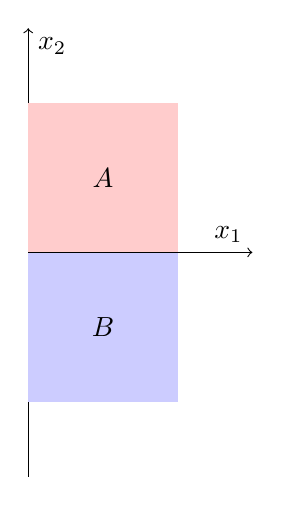
\begin{tikzpicture}
              \begin{axis}[ 
                ticks=none,
                axis lines = middle,
                axis line style={->},
                ymin=-1.5, ymax=1.5,
                xmin=0, xmax=1.5,
                xlabel={$x_{1}$},
                ylabel={$x_{2}$},
                axis equal image,
                disabledatascaling
                ]
                \fill [color=red!20] (0.0,0.001) rectangle (1,1);
                \fill [color=blue!20] (0.0,-0.001) rectangle (1,-1);
                \draw (0.5,0.5) node {$A$};
                \draw (0.5,-0.5) node {$B$};
              \end{axis}
            \end{tikzpicture}
          \end{figure}
        \end{minipage}
        \begin{minipage}{.45\textwidth}
          \[ A = \left\{ (x,+y) \mid x \in \interval[open]{0}{1} \wedge y\in \interval[open]{0}{1} \right\} \]
          \[ A = \left\{ (x,-y) \mid x \in \interval[open]{0}{1} \wedge y\in \interval[open]{0}{1} \right\} \]
        \end{minipage}
        
        Het is duidelijk dat $A$ en $B$ beide niet gesloten zijn, maar wel begrensd.
        $\delta$ is toch $0$:
        \[ \delta = \inf \{ \|a-b\| \mid a \in A, b \in B \} = \inf \interval[open]{0}{\sqrt{5}} \]
      \end{proof}
    \end{itemize}
  \item In willekeurige metrische ruimten bestaat er geen norm, maar we kunnen de stelling herformuleren als volgt:
    Zij $A$ en $B$ twee niet-lege, onderling disjuncte delen van een metrische ruimte $X,d$ en benoem $\delta$ als volgt:
    \[ \delta = \inf \{ d(a,b) \mid a\in A, b\in B \} \]
    Zelfs dan gaat de bewering niet op:
    \begin{proof}
      Beschouw de verzamelingen $A = \{ F_{2n} \mid n \in \mathbb{N}_{0} \}$ en $B = \{ F_{2n+1} \mid n\in \mathbb{N}_{0} \}$ in de metrische ruimte $\mathcal{F},h$ (uit voorbeeld \ref{vb:ttt-2-2014-1} op pagina \pageref{vb:ttt-2-2014-1}) 
      $A$ en $B$ zijn disjunct, begrensd en gesloten, maar $\delta$ zal toch $0$ zijn.
    \end{proof}
  \item Neem in plaats van $\mathbb{R}^{p}$ een willekeurige genormeerde vectorruimte en definieer de afstandsfunctie aan de hand van de norm.
    \extra{In een willekeurige genormeerde ruimte lijkt de stelling wel te gelden, bewijs}
  \end{enumerate}
  \feed
\end{st}

\begin{vb}
  \label{vb:bol-zonder-midden-samenhangend-in-hogere-dimensies}
  Kies $Y = \mathbb{R}^{p} \setminus \{0\}$.
  $Y$ is niet samenhangend voor $p=1$\vbref{vb:r_0-niet-samenhangend}, maar wel voor $p>1$.

  \begin{proof}
    We argumenteren dit voor $p=2$ (hogere dimensies gaan analoog).
    Beschouw de volgende convexe verzamelingen.
    \[ A_{1} = \{(x,y) \in \mathbb{R}^{2} \mid x > 0 \} \]
    \[ A_{2} = \{(x,y) \in \mathbb{R}^{2} \mid x < 0 \} \]
    \[ A_{3} = \{(x,y) \in \mathbb{R}^{2} \mid y > 0 \} \]
    \[ A_{4} = \{(x,y) \in \mathbb{R}^{2} \mid y < 0 \} \]
    Al deze verzamelingen zijn samenhangend \prref{pr:convexe-deelverzamelingen-samenhangend}
    $A_{1} \cap A_{3}$ is niet leeg en $A_{1} \cup A_{3}$ dus samenhangend.
    Analoog is $A_{2} \cup A_{4}$ samenhangend.
    Ook $A_{1} \cap A_{2}$ is leeg en $A_{1} \cup A_{2} \cup A_{3} \cup A_{4}$ samenhangend en dit is precies $\mathbb{R}^{2} \setminus \{0\}$.
  \end{proof}
\end{vb}

\begin{vb}
  Beschouw in $\mathbb{R}^{2}$ voor $n\in \mathbb{N}_{0}$ de verzameling $Y_{n}$ als volgt:
  \[ Y_{n} = \left\{ \left( x,\frac{x}{n} \right) \in \mathbb{R}^{2} \mid x\in \interval{0}{1} \right\} \]
  $Y_{n}$ is convex en dus samenhangend.
  Bovendien geldt $\bigcap Y_{n} = \{(0,0)\} \neq \emptyset$.
  De verzameling $Y = \bigcup Y_{n}$ is dus samenhangend.\prref{pr:niet-disjunctie-samenhangende-unie-samenhangend}
  Zij $L$ het lijnstuk met eindpunten $\left(\frac{1}{2},0\right)$ en $(1,0)$.
  $Y\cup L$ is samenhangend.
  
  \begin{proof}
    Bewijs uit het ongerijmde: Stel dat $Y \cup L$ niet samenhangend is.
    Er bestaan dan niet-lege, onderling gescheiden $A$ en $B$ zodat $Y\cup L = A \cup B$ geldt.
    Merk eerst op dat $L$ tot de sluiting van $Y$ behoort.
    Omdat $Y$ samenhangend is, moet $Y$ in zijn geheel tot ofwel $A$ ofwel $B$ behoren.
    Omdat $L$ tot de sluiting van $Y$ behoort moet $L$ tot $A$ behoren want $A$ en $B$ zijn onderling gescheiden.
    Er blijft dan niets meer over in $B$.
    Contradictie.
  \end{proof}
\end{vb}


\subsection{De $d_1$- of city block metriek op $\mathbb{R}^p$}
\label{sec:de-d_1-city}

\begin{vb}
  $\mathbb{R}^{p}$, uitgerust met de volgende functie als metriek, is een metrische ruimte:
  \[ d_{1}:\ \mathbb{R}^{p}\times\mathbb{R}^{p}\rightarrow (x,y) \mapsto d_{1}(x,y)=\sum_{i=1}^{p}|x_{i}-y_{i}| \]
  We noemen dit de \term{city block metriek} of \term{taxicab metriek}.
\extra{bewijs}
  \begin{figure}[H]
    \centering
    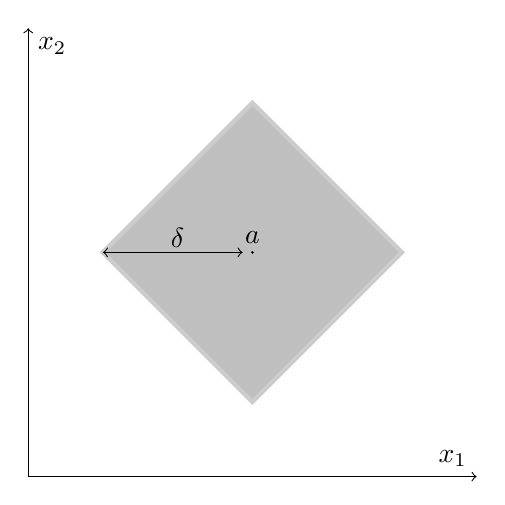
\begin{tikzpicture}
      \begin{axis}[ 
        ticks=none,
        axis lines = middle,
        axis line style={->},
        ymin=0, ymax=3,
        xmin=0, xmax=3,
        xlabel={$x_{1}$},
        ylabel={$x_{2}$},
        axis equal image,
        disabledatascaling
        ]
        \filldraw[ultra thick,fill=black!25!white, draw=black!20!white] (0.5,1.5) -- (1.5,2.5) -- (2.5,1.5) -- (1.5,0.5) -- cycle;
        \fill [fill=black] (1.5,1.5) circle [radius=0.01];
        \draw (1.5,1.6) node {$a$};
        \draw (1.5,1.5) node {} edge[<->] (0.5,1.5);
        \draw (1,1.6) node {$\delta$};
      \end{axis}
    \end{tikzpicture}
    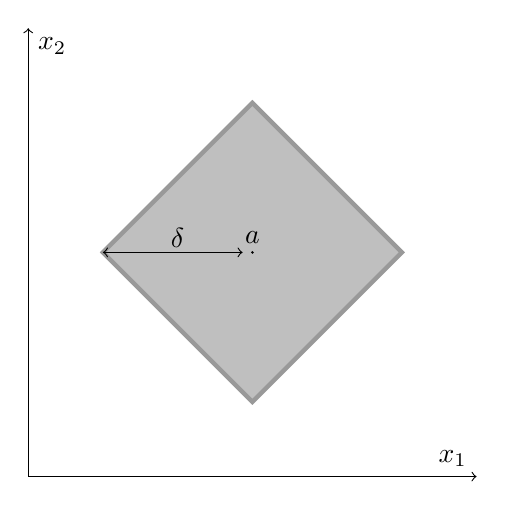
\begin{tikzpicture}
      \begin{axis}[ 
        ticks=none,
        axis lines = middle,
        axis line style={->},
        ymin=0, ymax=3,
        xmin=0, xmax=3,
        xlabel={$x_{1}$},
        ylabel={$x_{2}$},
        axis equal image,
        disabledatascaling
        ]
        \filldraw[ultra thick,fill=black!25!white, draw=black!40!white] (0.5,1.5) -- (1.5,2.5) -- (2.5,1.5) -- (1.5,0.5) -- cycle;
        \fill [fill=black] (1.5,1.5) circle [radius=0.01];
        \draw (1.5,1.6) node {$a$};
        \draw (1.5,1.5) node {} edge[<->] (0.5,1.5);
        \draw (1,1.6) node {$\delta$};
      \end{axis}
    \end{tikzpicture}
    \caption{Een open bol en een gesloten bol in $\mathbb{R}^{2},d_{1}$}
  \end{figure}
\end{vb}

\begin{st}
  $d$ en $d_{1}$ zijn topologisch equivalent op $\mathbb{R}^{p}$.

  \begin{proof}
    We moeten bewijzen dat er voor elke open bol $B(x,r)$ voor de gewone metriek een $d_{1}$-open bol $B_{1}(x,r_{1})$ bestaat met hetzelfde middelpunt die erin ligt en omgekeerd.
    \begin{itemize}
    \item $\Rightarrow$\\
      Kies een open bol $B(x,r)$ voor de gewone metriek.
      $B_{1}(x,r)$ voor de $d_{1}$ metriek is er dan een deel van:
      \[ \forall x,y\in A:\ d_{1}(x,y)^{2} = \left(\sum_{i=1}^{p}|x_{i}-y_{i}|\right)^{2} \ge \sum_{i=1}^{p}|x_{i}-y_{i}| = d(x,y)^{2} \]
      Als $d_{1}(x,y)$ dus kleiner is dan $r$ dan zal $d(x,y)$ dat ook zijn.

      \begin{figure}[H]
        \centering
        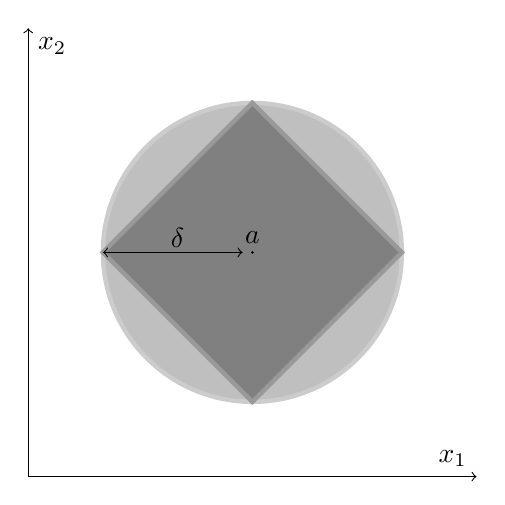
\begin{tikzpicture}
          \begin{axis}[ 
            ticks=none,
            axis lines = middle,
            axis line style={->},
            ymin=0, ymax=3,
            xmin=0, xmax=3,
            xlabel={$x_{1}$},
            ylabel={$x_{2}$},
            axis equal image,
            disabledatascaling
            ]
            \filldraw [ultra thick,fill=black!25!white, draw=black!20!white] (1.5,1.5) circle [radius=1];
            \filldraw[ultra thick,fill=black!50!white, draw=black!40!white] (0.5,1.5) -- (1.5,2.5) -- (2.5,1.5) -- (1.5,0.5) -- cycle;
            \fill [fill=black] (1.5,1.5) circle [radius=0.01];
            \draw (1.5,1.6) node {$a$};
            \draw (1.5,1.5) node {} edge[<->] (0.5,1.5);
            \draw (1,1.6) node {$\delta$};
          \end{axis}
        \end{tikzpicture}
        \caption{Een illustratie in $\mathbb{R}^{2}$}
      \end{figure}

    \item $\Leftarrow$\\
      Omgekeerd moeten we voor $r_{1}$ eenvoudigweg $\frac{r}{\sqrt{p}}$ nemen:
      \[ \forall x,y \in A:\ B_{1}(x,r) = \sum_{i=1}^{p}|x_{i}-y_{i}| \le \sqrt{\sum_{i=1}^{p}1} \sqrt{\sum_{i=1}^{p}|x_{i}-y_{i}|} = \sqrt{p}d(x,y) \]

      \begin{figure}[H]
        \centering
        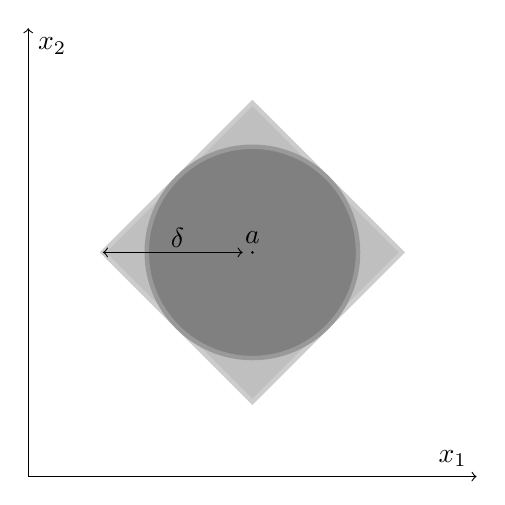
\begin{tikzpicture}
          \begin{axis}[ 
            ticks=none,
            axis lines = middle,
            axis line style={->},
            ymin=0, ymax=3,
            xmin=0, xmax=3,
            xlabel={$x_{1}$},
            ylabel={$x_{2}$},
            axis equal image,
            disabledatascaling
            ]
            \filldraw[ultra thick,fill=black!25!white, draw=black!20!white] (0.5,1.5) -- (1.5,2.5) -- (2.5,1.5) -- (1.5,0.5) -- cycle;
            \filldraw [ultra thick,fill=black!50!white, draw=black!40!white] (1.5,1.5) circle [radius=1/sqrt(2)];
            \fill [fill=black] (1.5,1.5) circle [radius=0.01];
            \draw (1.5,1.6) node {$a$};
            \draw (1.5,1.5) node {} edge[<->] (0.5,1.5);
            \draw (1,1.6) node {$\delta$};
          \end{axis}
        \end{tikzpicture}
        \caption{Een illustratie in $\mathbb{R}^{2}$}
      \end{figure}
    \end{itemize}
  \end{proof}
\end{st}


\subsection{De $d_\infty$- of maximummetriek op $\mathbb{R}^p$}
\label{sec:de-d_infty-maxim}

\begin{vb}
  $\mathbb{R}^{p}$, uitgerust met de volgende functie als metriek, is een metrische ruimte:
  \[ d_{\infty}:\ \mathbb{R}^{p}\times\mathbb{R}^{p}\rightarrow (x,y) \mapsto d_{\infty}(x,y)=\max_{i}|x_{i}-y_{i}| \]
  We noemen dit de \term{maximummetriek}.
\extra{bewijs}
  \begin{figure}[H]
    \centering
    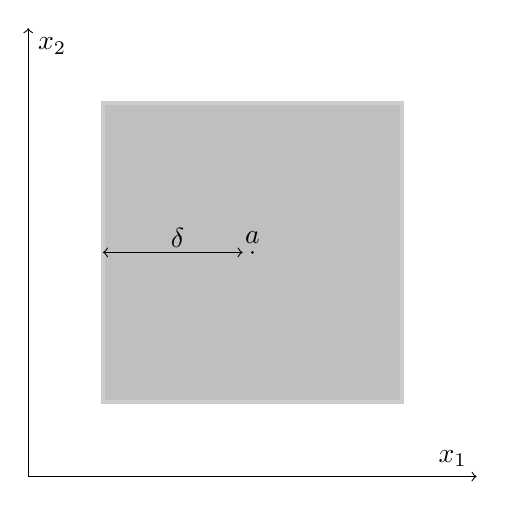
\begin{tikzpicture}
      \begin{axis}[ 
        ticks=none,
        axis lines = middle,
        axis line style={->},
        ymin=0, ymax=3,
        xmin=0, xmax=3,
        xlabel={$x_{1}$},
        ylabel={$x_{2}$},
        axis equal image,
        disabledatascaling
        ]
        \filldraw[ultra thick,fill=black!25!white, draw=black!20!white] (0.5,2.5) -- (2.5,2.5) -- (2.5,0.5) -- (0.5,0.5) -- cycle;
        \fill [fill=black] (1.5,1.5) circle [radius=0.01];
        \draw (1.5,1.6) node {$a$};
        \draw (1.5,1.5) node {} edge[<->] (0.5,1.5);
        \draw (1,1.6) node {$\delta$};
      \end{axis}
    \end{tikzpicture}
    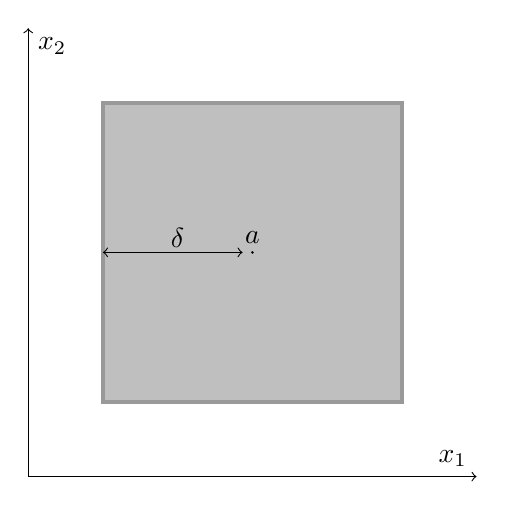
\begin{tikzpicture}
      \begin{axis}[ 
        ticks=none,
        axis lines = middle,
        axis line style={->},
        ymin=0, ymax=3,
        xmin=0, xmax=3,
        xlabel={$x_{1}$},
        ylabel={$x_{2}$},
        axis equal image,
        disabledatascaling
        ]
        \filldraw[ultra thick,fill=black!25!white, draw=black!40!white] (0.5,2.5) -- (2.5,2.5) -- (2.5,0.5) -- (0.5,0.5) -- cycle;
        \fill [fill=black] (1.5,1.5) circle [radius=0.01];
        \draw (1.5,1.6) node {$a$};
        \draw (1.5,1.5) node {} edge[<->] (0.5,1.5);
        \draw (1,1.6) node {$\delta$};
      \end{axis}
    \end{tikzpicture}
    \caption{Een open bol en een gesloten bol in $\mathbb{R}^{2},d_{\infty}$}
  \end{figure}
\end{vb}

\begin{st}
  $d$ en $d_{1}$ zijn topologisch equivalent op $\mathbb{R}^{p}$.

  \begin{proof}
    We moeten bewijzen dat er voor elke open bol $B(x,r)$ voor de gewone metriek een $d_{\infty}$-open bol $B_{\infty}(x,r_{1})$ bestaat met hetzelfde middelpunt die erin ligt en omgekeerd.
    \begin{itemize}
    \item $\Leftarrow$\\
      Kies $r_{\infty} = \frac{1}{\sqrt{p}}r$:
      \extra{bewijs}

      \begin{figure}[H]
        \centering
        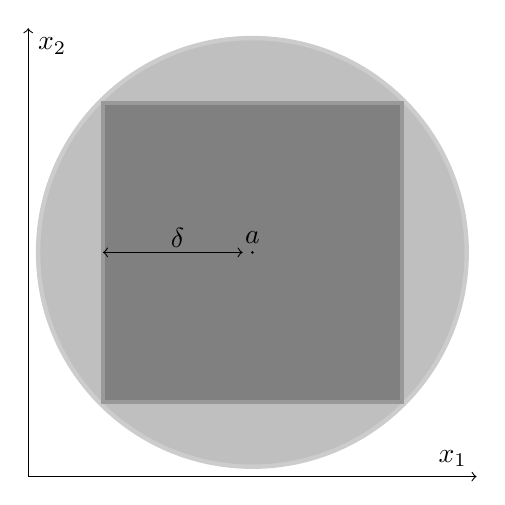
\begin{tikzpicture}
          \begin{axis}[ 
            ticks=none,
            axis lines = middle,
            axis line style={->},
            ymin=0, ymax=3,
            xmin=0, xmax=3,
            xlabel={$x_{1}$},
            ylabel={$x_{2}$},
            axis equal image,
            disabledatascaling
            ]
            \filldraw [ultra thick,fill=black!25!white, draw=black!20!white] (1.5,1.5) circle [radius=sqrt(2)+0.02];
            \filldraw[ultra thick,fill=black!50!white, draw=black!40!white] (0.5,2.5) -- (2.5,2.5) -- (2.5,0.5) -- (0.5,0.5) -- cycle;
            \fill [fill=black] (1.5,1.5) circle [radius=0.01];
            \draw (1.5,1.6) node {$a$};
            \draw (1.5,1.5) node {} edge[<->] (0.5,1.5);
            \draw (1,1.6) node {$\delta$};
          \end{axis}
        \end{tikzpicture}
        \caption{Een illustratie in $\mathbb{R}^{2}$}
      \end{figure}

    \item $\Rightarrow$\\
      Kies $r = r_{\infty}$:
      \extra{bewijs}

      \begin{figure}[H]
        \centering
        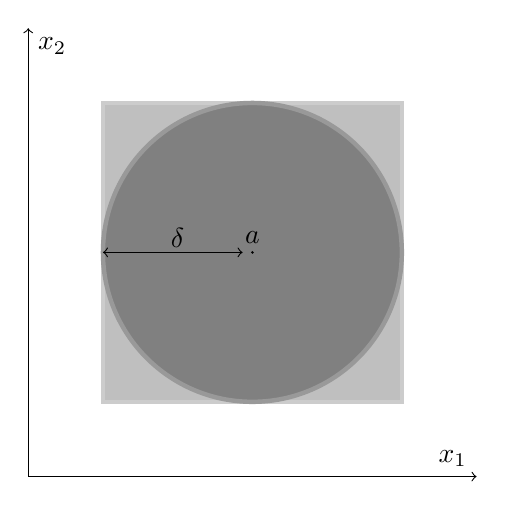
\begin{tikzpicture}
          \begin{axis}[ 
            ticks=none,
            axis lines = middle,
            axis line style={->},
            ymin=0, ymax=3,
            xmin=0, xmax=3,
            xlabel={$x_{1}$},
            ylabel={$x_{2}$},
            axis equal image,
            disabledatascaling
            ]
            \filldraw[ultra thick,fill=black!25!white, draw=black!20!white] (0.5,2.5) -- (2.5,2.5) -- (2.5,0.5) -- (0.5,0.5) -- cycle;
            \filldraw [ultra thick,fill=black!50!white, draw=black!40!white] (1.5,1.5) circle [radius=1];
            \fill [fill=black] (1.5,1.5) circle [radius=0.01];
            \draw (1.5,1.6) node {$a$};
            \draw (1.5,1.5) node {} edge[<->] (0.5,1.5);
            \draw (1,1.6) node {$\delta$};
          \end{axis}
        \end{tikzpicture}
        \caption{Een illustratie in $\mathbb{R}^{2}$}
      \end{figure}

    \end{itemize}
  \end{proof}
\end{st}


\subsection{De spoorwegmetriek op $\mathbb{R}^p$}
\label{sec:de-spoorw-op}

\begin{vb}
  $\mathbb{R}^{p}$, uitgerust met de volgende functie als metriek, is een metrische ruimte:
  \[
  d_{NMBS}:\ \mathbb{R}^{p}\times\mathbb{R}^{p}\rightarrow (x,y) \mapsto d_{NMBS}(x,y)=
  \begin{cases}
    \|x-y\| &\text{ als $x$ en $y$ lineair afhankelijk zijn}\\
    \|x\|+\|y\| &\text{ als $x$ en $y$ lineair onafhankelijk zijn}
  \end{cases}
  \]
  We noemen dit de \term{spoorwegmetriek}.
\extra{bewijs}
  \begin{figure}[H]
    \centering
    \begin{tikzpicture}
      \begin{axis}[ 
        ticks=none,
        axis lines = middle,
        axis line style={->},
        ymin=-1.5, ymax=2.5,
        xmin=-1.5, xmax=2.5,
        xlabel={$x_{1}$},
        ylabel={$x_{2}$},
        axis equal image,
        disabledatascaling
        ]
        \filldraw [ultra thick,fill=black!25!white, draw=black!20!white] (0,0) circle [radius=0.5];
        \fill [fill=black] (0.55,0.1) circle [radius=0.02];
        \draw [(-,color=black] (1.65,0.3) -- (0,0);
        \draw (0.55,0.2) node {$a$};
      \end{axis}
    \end{tikzpicture}
    \begin{tikzpicture}
      \begin{axis}[ 
        ticks=none,
        axis lines = middle,
        axis line style={->},
        ymin=0, ymax=2.5,
        xmin=0, xmax=2.5,
        xlabel={$x_{1}$},
        ylabel={$x_{2}$},
        axis equal image,
        disabledatascaling
        ]
        \fill [fill=black] (1.0,0.5) circle [radius=0.01];
        \draw [(-),color=black] (0.5,0.25) -- (1.5,0.75);
        \draw (1.1,0.4) node {$a$};
      \end{axis}
    \end{tikzpicture}
    \caption{Twee open bollen in $\mathbb{R}^{2},d_{NMBS}$ van verschillende straal}
  \end{figure}
\end{vb}

\begin{st}
  De spoorwegmetriek is topologisch fijner dan de gewone metriek.
  
  \begin{proof}
    Kies twee willekeurige elementen $x,y \in \mathbb{R}^{p}$:\stref{st:fijner-itv-afstanden}
    \[ d_{NMBS}(x,y) \ge \|x-y\| = d(x,y) \]
  \end{proof}
\end{st}


\end{document}

%%% Local Variables:
%%% mode: latex
%%% TeX-master: t
%%% End:
